%%%%% Schwingungen %%%%%
%% 1.1 Definitionen %%


%Some sample text to be displayed above the first subsection

%\subsection{Zyklotron}

%Ein Zyklotron besteht aus Zwei hohlen, halbzylindrischen und Duanden an denen eine Spannung mit unterschiedlichem Vorzeichen anliegt, und darüber bzw. darunter liegende Magneten, die ein homogenes Magnetfeld erzeugen. Zudem gibt es einen Einlass und einen Auslass für Teilchen.

%\begin{wrapfigure}{r}{0.4\textwidth} \label{Zyklo}
%
%	\vspace{-10pt}
%	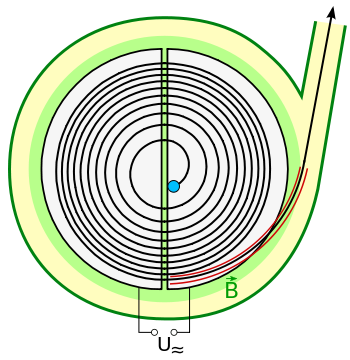
\includegraphics[width=0.35\textwidth]{Zyklotron_Prinzipskizze02.png}
%	\vspace{-13pt}
%	\caption{Prinzipskizze eines Zyklotrons}
%	\vspace{-5pt}	
%	
%\end{wrapfigure}

%\subsubsection{Anwendung}

% Some Formula:

%\begin{equation}
%	x= \frac{y \cdot 13 \pi z}
%			{\cos \alpha}
%\end{equation}


%%%%%%%%%%%%%%%%%%%%%%%%%%%
%%% Eigentlicher Beginn %%%
%%%%%%%%%%%%%%%%%%%%%%%%%%%

\subsection{Definitionen zu Schwingungen} \label{subsec:definitionenzuschwingungen}

Eine Schwingung bezeichnet eine periodische Energieumwandlung von einer in eine anderer Form von Energie und umgekehrt. \referenz{subsec:kenngroessen_schwingungen}


\subsubsection{Harmonische Schwingung}

Der zeitliche Verlauf einer harmonische Schwingung kann mit einer Sinuswelle beschrieben werden. Das mathematische Kriterium ist die Proportionalität der Rückstellkraft $F_{r}$ zum Betrag der Auslenkung $l$:

\begin{equation} \label{eq:kriterium_harmonisch}
	F_{r} \sim l
\end{equation}


\subsubsection{Schwingung}

Bei einer gedämpften Schwingung nimmt die Elongation über der Zeit ab. Außerhalb des im Physikunterricht angenommenen Modells sind alle Schwingung gedämpft, da Energie auch an die Umgebung abgegeben wird, beispielsweise durch Reibung in thermische Energie.



\subsection{Definitionen zu Wellen}

Als Welle bezeichnet man einen Vorgang bei dem Energie aber keine Masse transportiert wird. Es handelt sich um ein System gekoppelter Oszillatoren bei dem die Energie, die bei der Anregung eines Oszillators aufgewendet wird, vom diesem an die anderen Oszillatoren abgegeben wird. Daher wird die Energie räumlich transportiert, obwohl, absolut gesehen, sich jeder Oszillator noch stets an seinem Platz befindet.

\subsubsection{Transversalwelle}

Eine Transversalwelle ist eine Welle, deren Auslenkungsvektoren (= Richtung der Auslenkung) senkrecht auf der Ausbreitungsrichtung stehen.

Bsp.: Seilwelle, elektromagnetische Wellen (bei $ 400nm \leq \lambda \leq 700nm $: Licht)

\subsubsection{Longitudinalwelle}

Eine Longitudinal ist eine Welle, deren Auslenkungsvektoren (= Richtung der Auslenkung) parallel auf der Ausbreitungsrichtung stehen.

Bsp.: Schallwellen














